\subsection{Evaluation Datasets and Models}

We evaluated our experiments on six datasets. \textbf{SST2} \cite{socher-etal-2013-recursive} \textbf{SST5} \cite{socher-etal-2013-recursive}, \textbf{MR} \cite{10.3115/1219840.1219855} and \textbf{Subj} \cite{10.3115/1218955.1218990} are four datasets for sentiment classification; \textbf{AGNews} \cite{NIPS2015_250cf8b5} is a topic classification dataset; and \textbf{CB} \cite{Marneffe2019TheCI} is used
for natural language inference.
In our experiments, we use the same GPT-like pretrained language models used by \cite{dai2023gpt} with 1.3B released by fairseq\footnote{\url{https://github.com/facebookresearch/fairseq}}. 

\subsection{Evaluation Metrics}

The following sections describe the evaluation metrics adopted from \cite{dai2023gpt} to compare the behavior of ICL and finetuning.
% \paragraph{Prediction Recall}

% From the perspective of model prediction, models with similar behavior should have aligned predictions.
% We measure the recall of correct ICL predictions to correct finetuning predictions.
% Given a set of test examples, we count the subsets of examples correctly predicted by each model: $C_{\text{ZSL}}, C_{\text{ICL}}, C_{\text{FT}}$.
% To compare the update each method induces to the model's prediction we subtract correct predictions made in the ZSL setting.
% Finally we compute the \textbf{Rec2FTP} score as: $\frac{ \sizeof{ \left( C_{\text{ICL}} \cap C_{\text{FT}} \right) \setminus C_{\text{ZSL}} } }{ \sizeof{ C_{\text{FT}} \setminus C_{\text{ZSL}} } }$ .
% A higher Rec2FTP score suggests that ICL covers more correct behavior of finetuning from the perspective of the model prediction.
%This measure is agnostic to the inner workings of the attention mechanism.

\paragraph{Attention Output Direction (SimAOU)}
This metrics quantifies the similarity between two updates to the attention output of a layer with respect to the zero-shot setting. 
For a given query example, let $h^{(l)}_X$ represent the normalized output representation of the last token at the $l$-th attention layer within setting $X$.
The updates induced by ICL and finetuning are given by $h^{(l)}_{\text{ICL}} - h^{(l)}_{\text{ZSL}}$ and $h^{(l)}_{\text{FT}} - h^{(l)}_{\text{ZSL}}$, respectively.
The attention output similarity (\textbf{SimAOU}) is defined to be the cosine similarity between these updates averaged across all layers.
A higher SimAOU score indicates that ICL is more inclined to adjust the attention output in the same direction as finetuning.
For the sake of comparison, this score is compared with a baseline of SimAOU with random attention output updates: $h^{(l)}_{\text{rand}} - h^{(l)}_{\text{ZSL}}$ where $h^{(l)}_{\text{rand}}$ is sampled uniformly.

\paragraph{Attention Map Similarity}
We use SimAM to measure the similarity between attention maps and query tokens for ICL and finetuning.
For a query example, let $m^{(l,h)}_X$ represent the attention weights before softmax in the $h$-th head of the $l$-th layer for setting $X$. In ICL, we focus solely on query token attention weights, excluding demonstration tokens. Initially, before finetuning, we compute the cosine similarity between $m^{(l,h)}_{\text{ICL}}$ and $m^{(l,h)}_{\text{ZSL}}$, averaging it across attention heads to obtain SimAM (Before Finetuning) for each layer.
Similarly, after finetuning, we calculate the cosine similarity between $m^{(l,h)}_{\text{ICL}}$ and $m^{(l,h)}_{\text{FT}}$ to obtain SimAM (After FT). A higher SimAM (After FT) relative to SimAM (Before FT) indicates that ICL's attention behavior aligns more with a finetuned model than a non-finetuned one.


\subsection{ICL Predictions Poorly Align with Finetuning}
\begin{figure*}[h!]
  \centering
  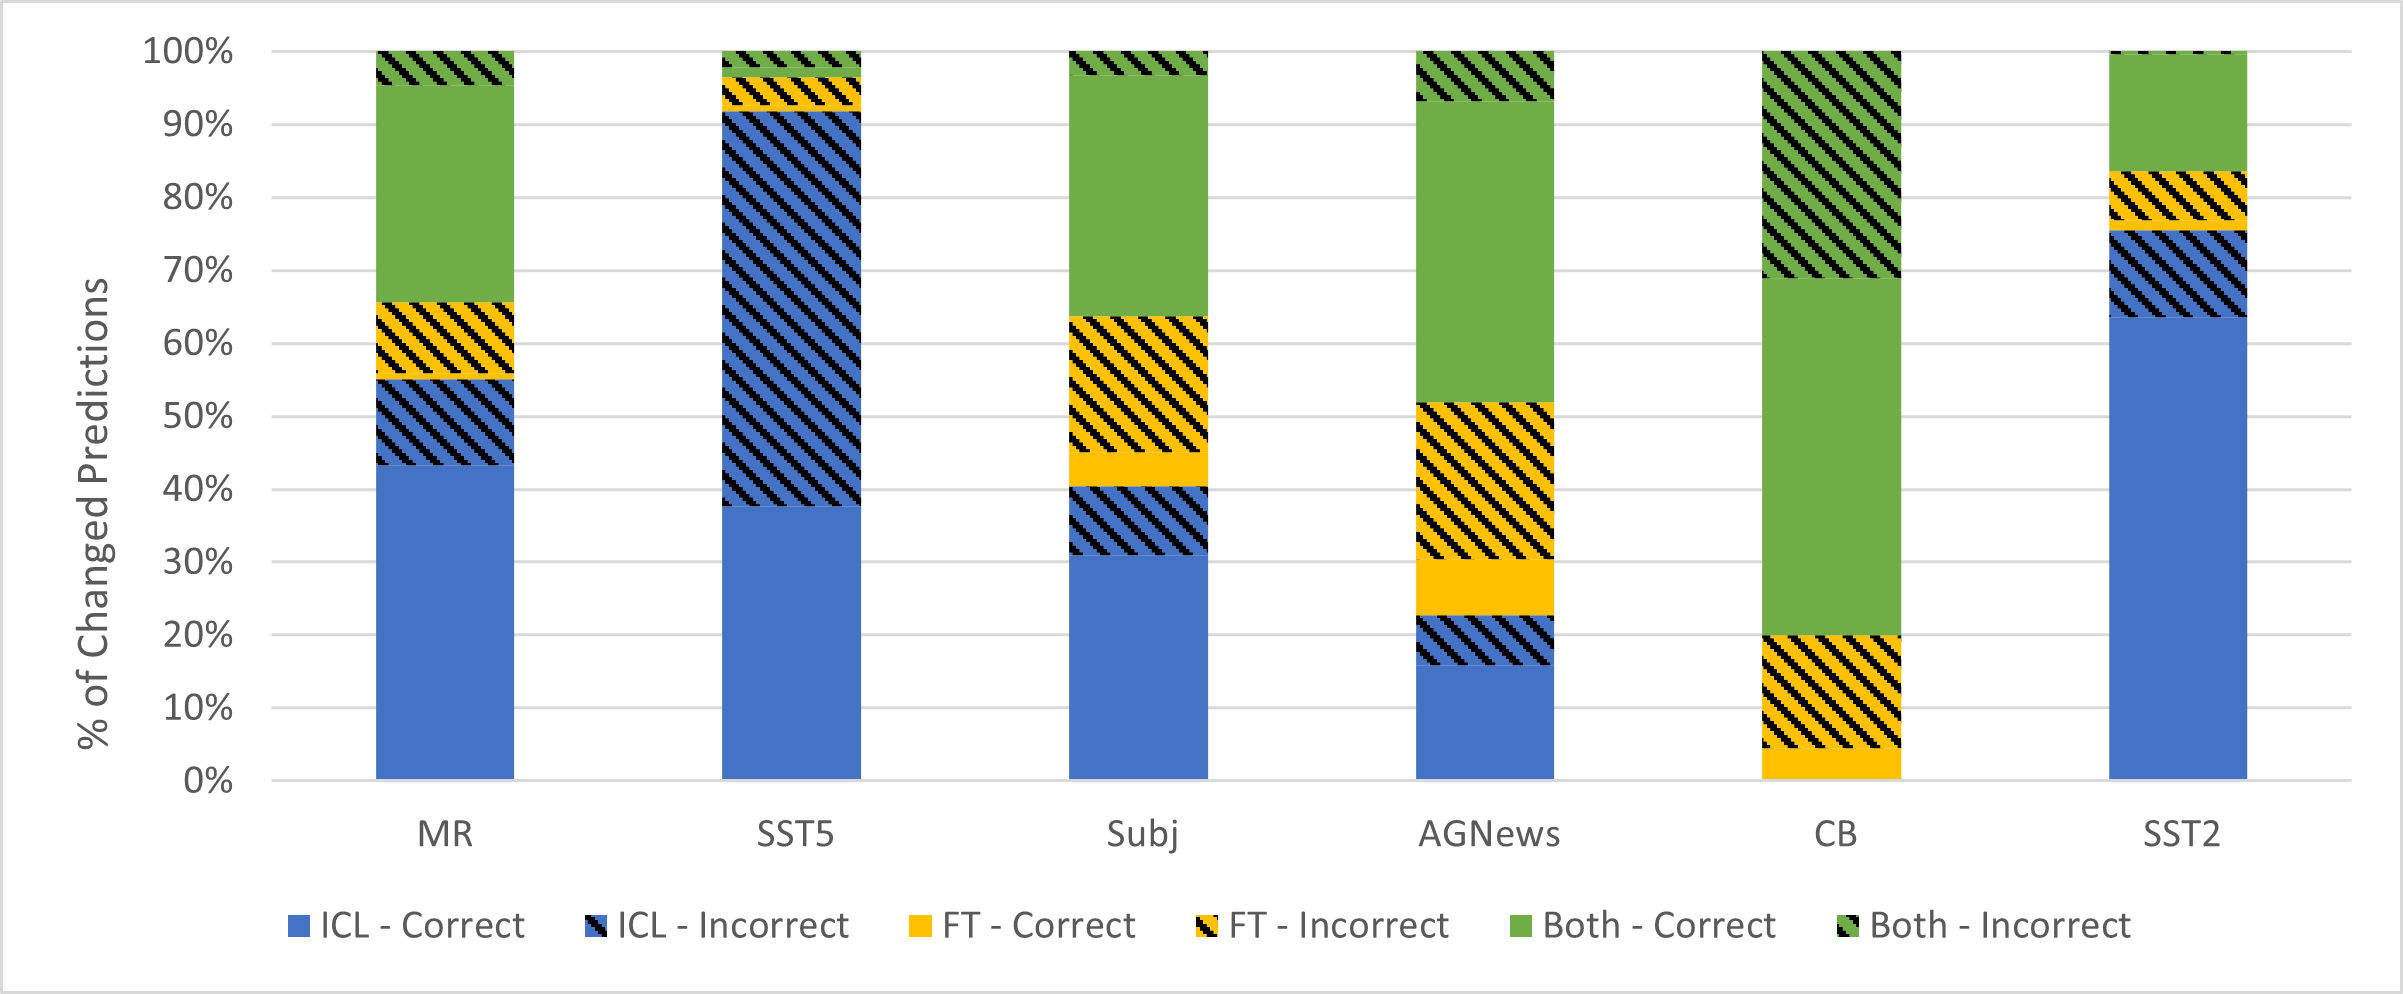
\includegraphics[width=0.98\linewidth,height=6cm]{resources/images/prediction_alignment.png}
  \caption{
    Partition of prediction changes with regards to the zero-shot setting induced by ICL and FT.
    For each task, we evaluate both methods on the same validation set.
    Correct changes are examples that are misclassified in the ZSL setting and are correctly classified following the prediction update.
    incorrect changes are examples whose prediction is changed from the ZSL setting into an incorrect label.
  }
  \label{fig:prediction_alignment}
\end{figure*}
\begin{table*}[ht!]
  \centering
  \setlength{\tabcolsep}{7pt}
  \begin{tabular}{l | c c c c c c}
  \toprule
  & \textbf{CB} & \textbf{SST2} & \textbf{SST5} & \textbf{Subj} & \textbf{MR} & \textbf{AGNews} \\ 
  \midrule
   ZSL Accuracy & 37.5 & 70.5 & 39.3 & 72.6 & 65.9 & 46.2 \\
   FT Accuracy & 57.1 & 74 & 39.4 & 77.8 & 72.6 & 66.7 \\
   ICL Accuracy & 50 & 92.7 & 45.0 & 90.0 & 89.1 & 79.2 \\
  \midrule
  RPA (\%)           & 80.0 & 16.4 & 3.4 & 36.2 & 34.0 & 48.0 \\
  RPA - Correct (\%) & 91.7 & 19.8 & 3.2 & 48.0 & 40.2 & 63.5 \\
  RPA - Incorrect (\%) & 66.7 & 1.8 & 3.5 & 10.2 & 17.7 & 19.2 \\
  \end{tabular}
  \caption{Validation accuracy and RPA scores for ZSL, finetuning, and ICL settings on all six classification datasets.}
  \label{tab:acc_rpa}
\end{table*}
In this section we focus on the perspective of model predictions, regarding both ICL and finetuning as black-box updates to the original zero-shot prediction.
While this analysis provides less insight into the inner workings of ICL, prediction alignment is easily interpretable and seems necessary for downstream applications of such comparisons.

Revisiting the results of \cite{dai2023gpt}, the authors find that find that ICL achieves high recall to finetuning (Rec2FTP) scores across multiple tasks, which means it covers most of the correct predictions of finetuning. 
However their results show a discrepancy between the accuracy of the finetuned model and the ICL setting, average difference of $\textbf{19.38\%}$ relative to the original zero-shot accuracy (Table \ref{tab:acc_rpa}).


We argue that Rec2FTP is insufficient to quantify prediction alignment in this setting because:
(1) it does not the difference between the number of changes induced by each method;
(2) it does not account for incorrect prediction changes.
Figure \ref{fig:prediction_alignment} shows the number of prediction updates induced by each method.
The results show that overall ICL is more inclined to change the ZSL prediction.
Note that although ICL covers almost all FT correct prediction changes (high Rec2FTP), in most tasks unique FT and to ICL predictions constitute the majority of all updates.
This observation shows the importance of measuring incorrect prediction changes as well.

We propose a metric that respects these factors: \textbf{relative prediction alignment} (RPA) to quantify prediction alignment in this setting.
Given a validation set, we denote the subset of example whose prediction is changed with regards to the zero-shot setting by ICL or FT by $D_\text{ICL}$ and $D_\text{FT}$ respectively.
We define the RPA of these updates by: 
\begin{equation*}
  \text{RPA}_{D_\text{ICL}, D_\text{FT}} = \frac{\sizeof{D_\text{ICL} \cap D_\text{FT}}}{\sizeof{D_\text{ICL}} + \sizeof{D_\text{FT}} - \sizeof{D_\text{ICL} \cap D_\text{FT}}} 
\end{equation*}

We report the RPA scores across all tasks in table \ref{tab:acc_rpa}.
For each we also compute the RPA scores computed over only for prediction changes to correct labels, and those for incorrect labels.
The results show that correct prediction changes are more aligned between the two methods.


\subsection{Layer Causality in Finetuning}
\label{sec:layer_causality}
\begin{figure}[h]%
	\centering
	\subfloat{{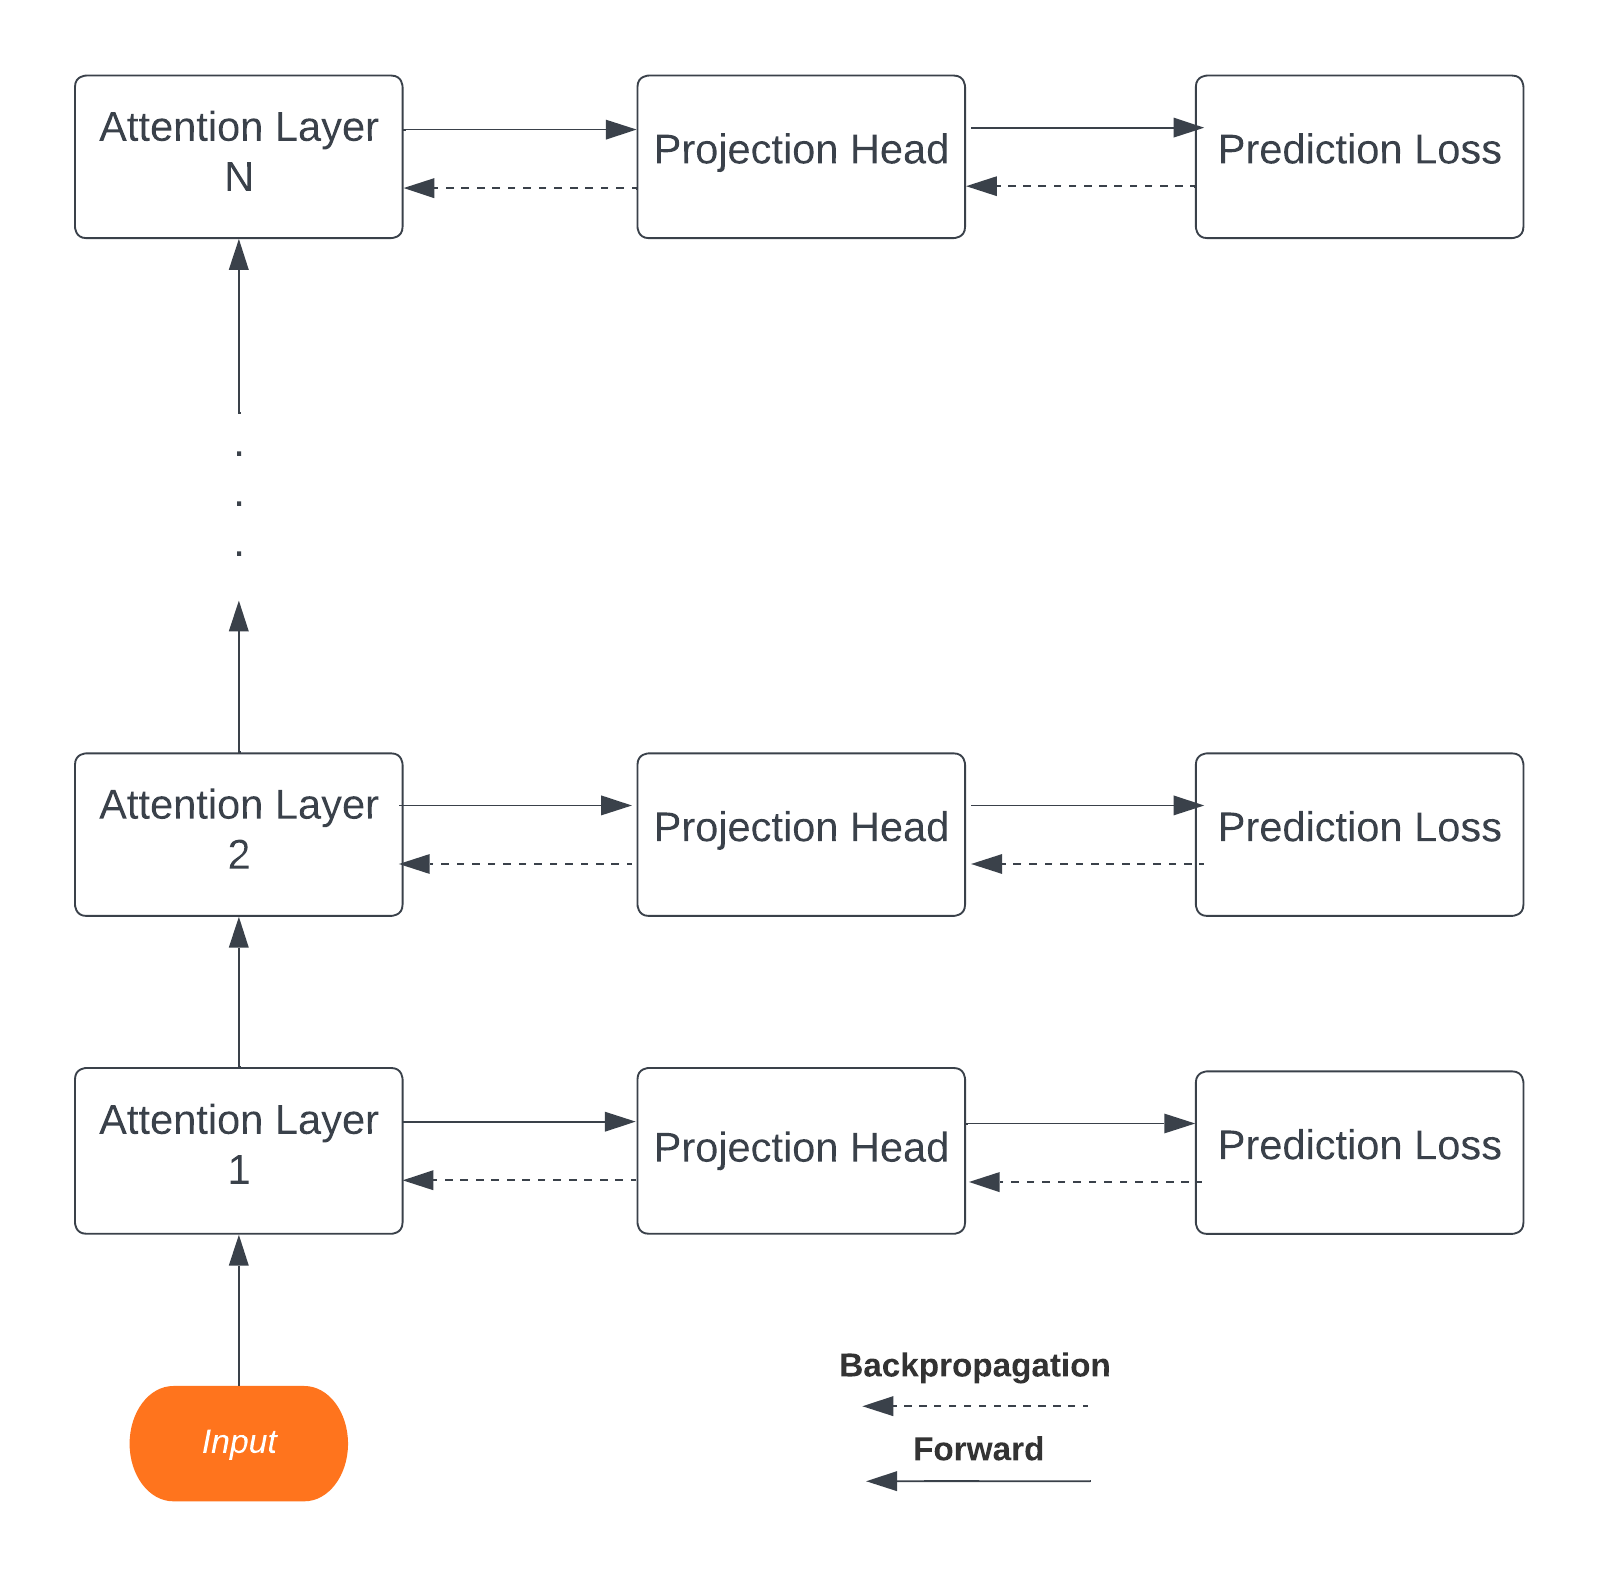
\includegraphics[width=8cm]{resources/images/causal_layer_diagram.png}}}%
	\caption{\textbf{Layer-Causal Finetuning}: The output of each layer is projected to the label space and used as an intermediate prediction.
		We compute the prediction loss of each intermediate layer sequentially.
	}
	\label{fig:layer_causal_diagram}
\end{figure}
\begin{table*}[h!]
	\centering
	\setlength{\tabcolsep}{7pt}
		\begin{tabular}{l| c c c c c c c }
			\toprule
			& \textbf{SST2} & \textbf{SST5} & \textbf{MR} & \textbf{Subj} & \textbf{AGNews} & \textbf{CB} & \textbf{Average}         \\
			\midrule
			 SimAOU (Random)        & 0.0016 & 0.0025 & 0.0008 & 0.0022 & 0.0021 & 0.0037 & 0.0021          \\
			 SimAOU (FT)            & 0.1091 & \textbf{0.113}  & 0.2190  & 0.1932  & 0.3053 & 0.2013 & 0.1901          \\
			 SimAOU (Layer Casual FT)  & \textbf{0.2297} & 0.1065 & \textbf{0.3299} & \textbf{0.3439} & \textbf{0.3213} & \textbf{0.3435} & \textbf{0.2791} \\
			 \midrule
			 SimAM (ZSL)                 & 0.5546 & 0.3913 & 0.3979 & 0.3786 & 0.1518 & 0.1524 & 0.3377          \\
			 SimAM (Standard FT)         & \textbf{0.5850}  & \textbf{0.4047} & \textbf{0.4980}  & \textbf{0.4870}  & \textbf{0.4944} & \textbf{0.1875} & \textbf{0.4427} \\
			 SimAM (Layer Causal FT)     & 0.5774 & 0.4039 & 0.2919 & 0.2844 & 0.1201 & 0.0293 & 0.2845          \\	
		\end{tabular}
		\caption{SimAOU and SimAM comparison of standard FT and layer causal FT across six classification datasets.
			Layer causal FT achieves higher SimAOU across 5 out of 6 tasks, yet its SimAM is significantly lower. 		
		}
		\label{tab:layer_causal}
\end{table*}
		

In this section we highlight an intrinsic difference in information flow of attention output updates between standard finetuning and ICL.

\begin{enumerate}
	\item \textbf{Layer Causality}: In ICL the update to the output of the $l$-th attention layer is dependent only on the output of previous (lower) layers.
  On contrast, the update to the $l$-th attention output induced by finetuning is determined by the gradient of the entire model's trainable parameters.
	
  \item \textbf{Sequential Update}: Equation \ref{equ:icl_opti_dual} shows that in ICL each attention layer's output is updated sequently throughout the model's depth axis.
  However, in GD based finetuning all layer's parameters are updated in a single concurrent step.
\end{enumerate}

Motivated by these observations we propose a layer causality aware finetuning method where each layer is updated individually.
Specifically, we project the output of each layer into the label space using the pertained projection head and compute the cross-entropy loss of this prediction.
% Check if this is implemented %
We update each layer sequentially, regarding the previous layers output as constant.  

We evaluate our method in comparison to standard finetuning using using the experiments proposed by \cite{dai2023gpt}.
Table~\ref{tab:layer_causal} shows the SimAOU and SimAM measurements of both methods in comparison to ICL.
Layer causal FT achieves higher SimAOU in 5 out of 6 tasks, but its SimAM is significantly lower.

We highlight two fallacies of our proposed method, and how they might have contributed to lower performance and SimAM scores.
\begin{itemize}
	\item Lower layers in the models are not trained to directly produce predictions, thus our FT method causes significant drift from the original models learned weights.
	\item The gradients applied to lower layers have bigger magnitude in layer causal FT.
				During pertaining the gradient of early layers is propagated throughout the model which usually dampens its norm.  
\end{itemize}

We verify this hypothesis by comparing the norm of  each attention layer's gradient during the standard FT process and layer causal FT in figure \ref{fig:grad_norm_comparison}.

\begin{figure*}%
	\centering
	\subfloat{{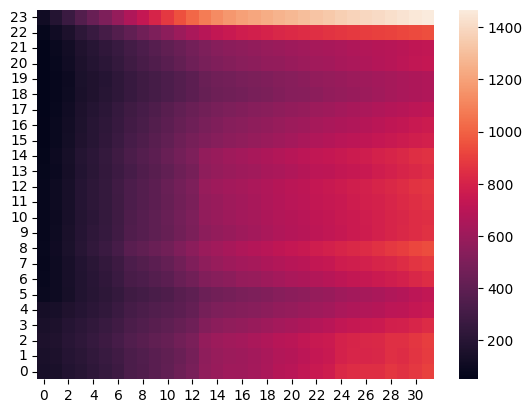
\includegraphics[width=6cm]{resources/images/full_ft_grad_norm.png}}}%
	\subfloat{{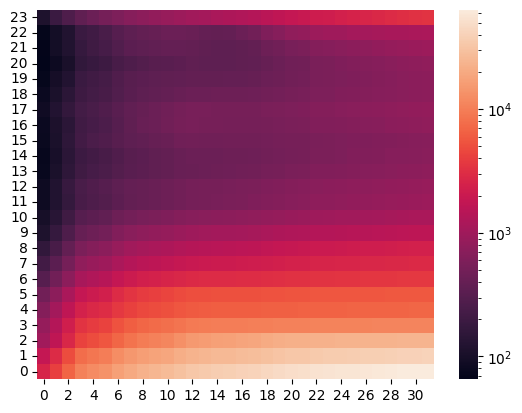
\includegraphics[width=6cm]{resources/images/causal_layer_grad_norm.png}}}%
	\caption{Heatmap of $\ell_2$ norms of the gradients computed during finetuning on the Subj task. Note the different scales of magnitude.
	 \textbf{Horizontal Axis}: training demonstration index. 
	 \textbf{Vertical Axis}: layer index in ascending order (from input to network output).
	 \textbf{Left}: Standard FT.
	 \textbf{Right}: Layer-Causal FT (norm magnitude in logarithmic scale).
	 }
	\label{fig:grad_norm_comparison}
\end{figure*}

Following this finding, we attempt to apply gradient clipping in the layer causal process with limited success.
We report preliminary results using a manually selected clip value on the Subj task in table~\ref{tab:per_layer_clipping_metrics}.
\begin{table*}[th]
	\centering
	\setlength{\tabcolsep}{7pt}
		\begin{tabular}{l | c}
		\toprule
		& \textbf{Subj} \\
		\midrule
		 SimAUO (Standard FT)     & 0.1932 \\
		 SimAUO (LC-FT Clipped)   & \textbf{0.3480}  \\
		\midrule
		 SimAM (ZSL)                     & 0.3786 \\
		 SimAM (Standard FT)             & \textbf{0.4870} \\
		 SimAM (LC-FT Clipped)           & 0.4227 \\
		
		\end{tabular}
	\caption{
		% Left shows the results for the per-layer training process. Middle shows the results for the per-layer training process with gradient norm clipping. Right shows the results for the standard fine-tuning process.
		Comparison of layer-causal finetuning with gradient norm clipping (clipped to 12.0 in $\ell_\infty$ norm).
		This results show that even arbitrary clipping may resolve the drop in SimAM shown in table \ref{tab:layer_causal}.
	}
	\label{tab:per_layer_clipping_metrics}
\end{table*}


\subsection{ICL Attention Update Expressiveness}
We calculated SimAOU and SimAM for both original and linearized models. Results are shown in Table \ref{tabel:lin_results}.
In addition we were unable evaluate the linearized model on the datasets AGNews and CB due to heavy memory consumption. 
The results indicate that the linearized model yields lower similarity scores compared to the original model but significantly higher scores than a random vector. This suggests that our hypothesis was incorrect and other simple model versions should be thought of. More on that in the discussion section.
\begin{table*}
	\centering
  \setlength{\tabcolsep}{7pt}
	\begin{tabular}{l | c c c c c }
    \toprule
    & SST2   & SST5   & MR     & Subj  & Average \\
		\midrule
    SimAOU (Random)   & 0.001  & 0.002  & 0.001  & 0.002 & 0.002          \\
		SimAOU (FT)       & 0.1091 & \textbf{0.113}  & \textbf{0.219}  & \textbf{0.193} & \textbf{0.158} \\
		SimAOU (FT Lin)   & \textbf{0.122}  & 0.0789 & 0.171  & 0.148 & 0.130          \\
    \midrule
    SimAM (Before FT)     & 0.5547 & 0.3914 & 0.398 & 0.378 & 0.430          \\
    SimAM (After FT)      & \textbf{0.585}  & \textbf{0.404}  & \textbf{0.498} & \textbf{0.487} & \textbf{0.493} \\
    SimAM (After FT Lin)  & 0.573  & 0.403  & 0.448 & 0.449 & 0.468          \\
  \end{tabular}

	\caption{
    SimAOU and SimAM comparison of standard FT and FT using the linear approximation of the model.	 		
  }
	\label{tabel:lin_results}
\end{table*}
